\section{Vision Transformer}
\label{section:transformer}
Transformer \cite{vaswani2017attention} revolutionized the field with its innovative approach to sequential, contextual modeling, primarily to solve the next word prediction task. The model architecture consists of two fundamental components, namely Positional Embedding and Attention Mechanisms, which are also widely used in other models, especially our concerning related works. For instance, Vision Transformer (ViT) built upon this groundwork \cite{dosovitskiy2020image} marked a significant milestone by demonstrating that a pure Transformer could outperform CNNs in image feature extraction. SegFormer \cite{xie2021segformer}, one of the models applied in our watermark removal pipeline, improves ineffective settings in ViT for semantic segmentation task.

In this section, we discuss in details the building blocks of Transformer. Then we finally summarize the architecture dataflow. Firstly, let us denote by $\mathbf{X}=(\xbf_1,\ldots, \xbf_N)\in\RR^{D\times N}$ the sequence of tokens fed to the input of the neural network.

\subsection{Positional Embedding}
Recurrent Neural Networks \cite{rumelhart1986learning} was the first attempt to model sequential data, especially for sentences in NLP tasks. Positional Embedding serves as an alternative for deep learning architectures so that the dataflow is fully feedforward. The method modifies each token $\xbf_n, n\in\{1,\ldots,N\}$ element-wise to reflect positional information by

\begin{equation}
  \xbf_n^{(d)} \leftarrow \xbf_n^{(d)} + \mathrm{PE}(n,d),
\end{equation}
where $\mathrm{PE}(n,d)$ is a positional encoding function, for $n\in\{1,\ldots,N\}$ and $d\in\{1,\ldots,D\}$. In Transformer, the authors hypothesized that the effect of each pair of tokens to each other depends on the distance between them i.e. for each $m\in\{1,\ldots,N\}$, there exists a linear transformation $\bm{\Phi}^{(m)}$ such that

\begin{equation}
  \bm{\Phi}^{(m)}\xbf_n = \xbf_{n+m},
\end{equation}

where $n\in\NN$ satisfying $0\le n+m\le N$. Hence, given that $D$ is even, they decided to use the sinusoid for positional encoding

$$\mathrm{PE}(n,d) =
  \begin{cases}
    \sin(\omega_k\cdot n), \text{ if } d = 2k \\
    \cos(\omega_k\cdot n), \text{ if } d = 2k+1,
  \end{cases}$$
where $\omega_k = \dfrac{1}{10000^{2k/D}}$.

Indeed, the function seamlessly meets their requirement. Consider two tokens $\xbf_n$ and $\xbf_{n+m}$, each at two dimensions $2k$ and $2k+1$. We aim to find a matrix $M^{(m)}_k=\begin{pmatrix}u_1 & u_2 \\ v_1 & v_2\end{pmatrix}\in\RR^{2\times2}$ such that
\begin{equation}
  \label{equation:sinusoid-transformation}
  M\begin{pmatrix}
    \sin(\omega_k\cdot n) \\
    \cos(\omega_k\cdot n)
  \end{pmatrix} = \begin{pmatrix}
    \sin(\omega_k\cdot (n+m)) \\
    \cos(\omega_k\cdot (n+m))
  \end{pmatrix}.
\end{equation}

Since
\begin{align*}
  \sin(\omega_k\cdot (n+m)) & = \sin(\omega_k\cdot n)\cos(\omega_k\cdot m) + \cos(\omega_k\cdot n)\sin(\omega_k\cdot m)  \\
  \cos(\omega_k\cdot (n+m)) & = \cos(\omega_k\cdot n)\cos(\omega_k\cdot m) - \sin(\omega_k\cdot n)\sin(\omega_k\cdot m).
\end{align*}

Plug the expansion into Equation \ref{equation:sinusoid-transformation}, we get the solution
\begin{equation}
  M^{(m)}_k =
  \begin{pmatrix}
    \cos(\omega_k\cdot m)  & \sin(\omega_k\cdot m)  \\
    -\sin(\omega_k\cdot m) & \sin(\omega_k\cdot m),
  \end{pmatrix}
\end{equation}
which only depends on $m$. Therefore, we have
\begin{equation}
  \begin{pmatrix}
    M^{(m)}_1 & 0      & \cdots & 0             \\
    0         & \ddots & \cdots & 0             \\
    0         & \cdots & 0      & M^{(m)}_{D/2}
  \end{pmatrix} \xbf_n = \xbf_{n+m}.
\end{equation}

\begin{figure}[ht]
  \centering
  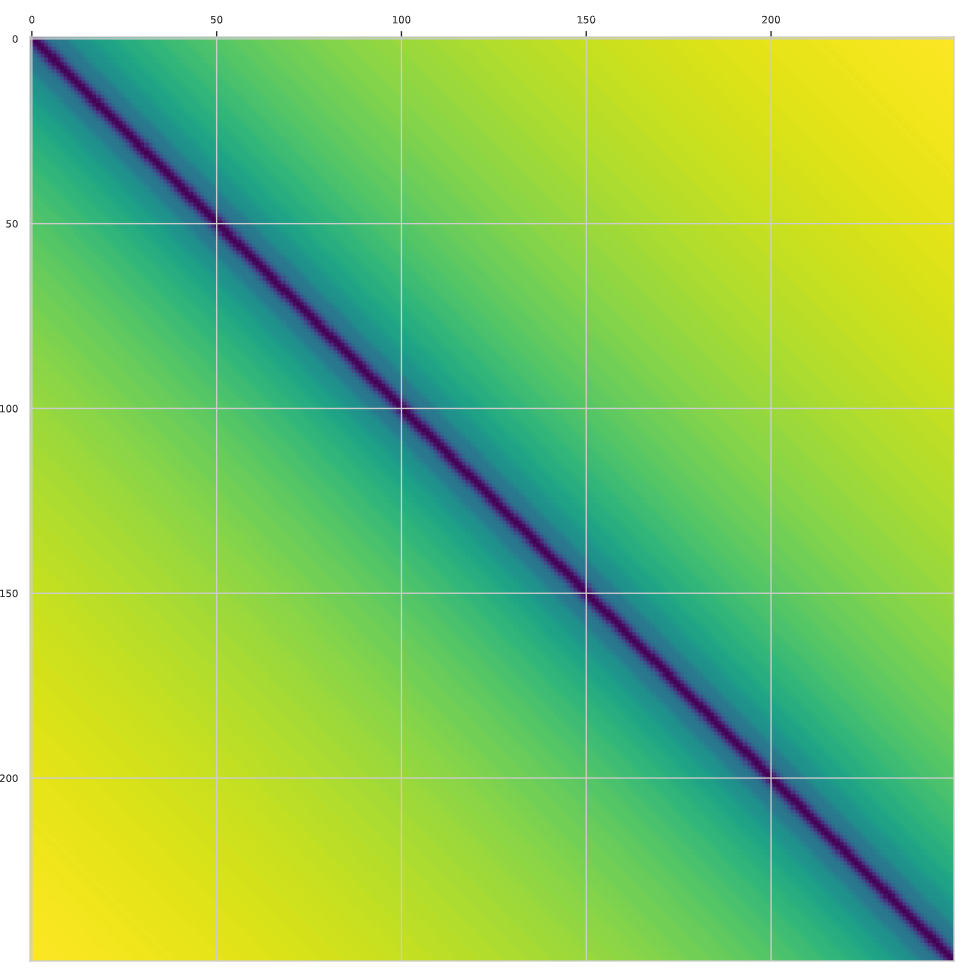
\includegraphics[width=0.6\textwidth]{img/positional-embedding-heatmap.png}
  \captionsetup{justification=centering} % Center the caption
  \caption[Positional embedding heatmap]{Positional embedding heatmap. Source \href{harrisonpim.com/blog/understanding-positional-embeddings-in-transformer-models}{Harrison Pim's blog}.}
  \label{figure:positional-embedding-heatmap}
\end{figure}

The effect of sinusoid positional embedding is illustrated in Figure \ref{figure:positional-embedding-heatmap}. We compute the dot product of every pair of token whose positions from $0$ to $250$. A darker color indicates a higher value of dot product. We can see a pattern that the heatmap gets brighter when going away from the diagonal, meaning that closer tokens are higher relevant.

\subsection{Attention Mechanisms}

Attention mechanisms are motivated by human volitional and nonvolitional cues \cite{zhang2023dive}. Let say while you are thirsty, there are three objects in front of you, a glass of orange juice, a politics newspaper and a deep learning book. Nonvolitionally, you pay attention to the orange juice. After you quenched, as a deep learning enthusiast, you deliberately take the deep learning book instead of the politics newspaper, which is an instance of volitional cues. Parameterized fully-connected layers or even non-parameterized layers like max or average pooling can be regarded as to bias selection over sensory inputs. The set of three given objects is called a \textit{context}. A nonvolitional state is called a \textit{key}. We may not capture all features of the context, for example, how the newspaper smells, but only a few sensory inputs depending on your nonvolitional state current mental and physical state, like the thirst in the example.  A sensory feature is called a \textit{value}, paired with a key. Attention mechanisms also model volitional cues, like your enthusiasm in deep learning, which in the language of attention mechanisms, is called a \textit{query}.

\begin{figure}[ht]
  \centering
  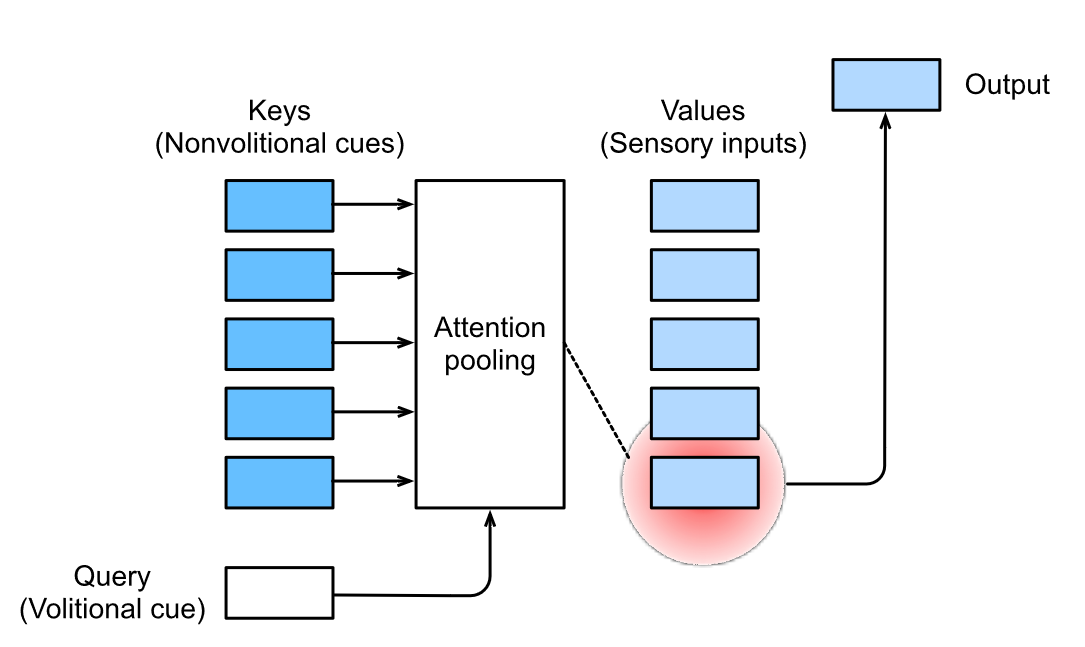
\includegraphics[width=0.75\linewidth]{img/attention.png}
  \vspace{0.25cm}
  \caption[Overview of Attention Mechanism]{Overview of Attention Mechanism \cite{zhang2023dive}}
  \label{figure:attention}
\end{figure}

Mathematically, a context includes a set of tokens after positional embedding, say $\mathbf{Y}=(\ybf_1,\ldots, \ybf_N)\in\RR^{D\times N}$. The tokens correspond to the values $\mathbf{V}=(\v_1,\ldots, \v_N)\in\RR^{D\times N}$, in result of the keys $\mathbf{K}=(\k_1,\ldots, \k_N)\in\RR^{d_k\times N}$. We also asset each token a query $\q_n, n\in\{1,\ldots,N\}$ and denote $\mathrm{Q} = (\q_1,\ldots, \q_N)$. A query effects more considerably on a token $\ybf_n, n\in\{1,\ldots,N\}$, if it highly matches the corresponding key $\k_n$. We model the matching score by dot product. For this reason, the queries are selected to have the same dimension as the keys. For each query $\q_n, n\in\{1,\ldots,N\}$, the authors computed the matching scores $\q_n \mathbf{K}^\top$, then normalized into $\mathrm{softmax}\left(\dfrac{\q_n\mathbf{K}^\top}{\sqrt{d}}\right)$.
More compactly,
\begin{equation}
  \mathrm{Attention}(\mathbf{Q}, \mathbf{K}, \mathbf{V}) = \mathrm{softmax}\left(\dfrac{\mathbf{Q}\mathbf{K}^\top}{\sqrt{d}}\right)\mathbf{V}.
\end{equation}
The authors used three learnable matrices $\mathbf{W_v}\in \RR^{D\times D}$, $\mathbf{W_k}\in \RR^{d_k\times D}$ and  $\mathbf{W_q}\in \RR^{d_k\times D}$ to extract the values, keys and queries from the tokens i.e.
$$\mathbf{V} = \mathbf{W_v}\mathbf{Y}, \mathbf{K} = \mathbf{W_k}\mathbf{Y} \text{ and } \mathbf{Q} = \mathbf{W_q}\mathbf{Y}.$$

In practice, the authors employed \textit{Multi-head Attention}. In instead of one value matrix, $h:=\dfrac{D}{d_v}$ value matrices $\mathbf{W_v}\in \RR^{D\times d_v}$ are used, where $d_v$ divides $D$, yielding $h$ $d_v$-dimensional output tokens in parallel. The outputs are then concatenated to $D$-dimensional tokens. In general, the keys and queries can be generated from two different sequence, which we called Cross Attention.

\subsection{Transformer Architecture}
\begin{figure}[ht]
  \centering
  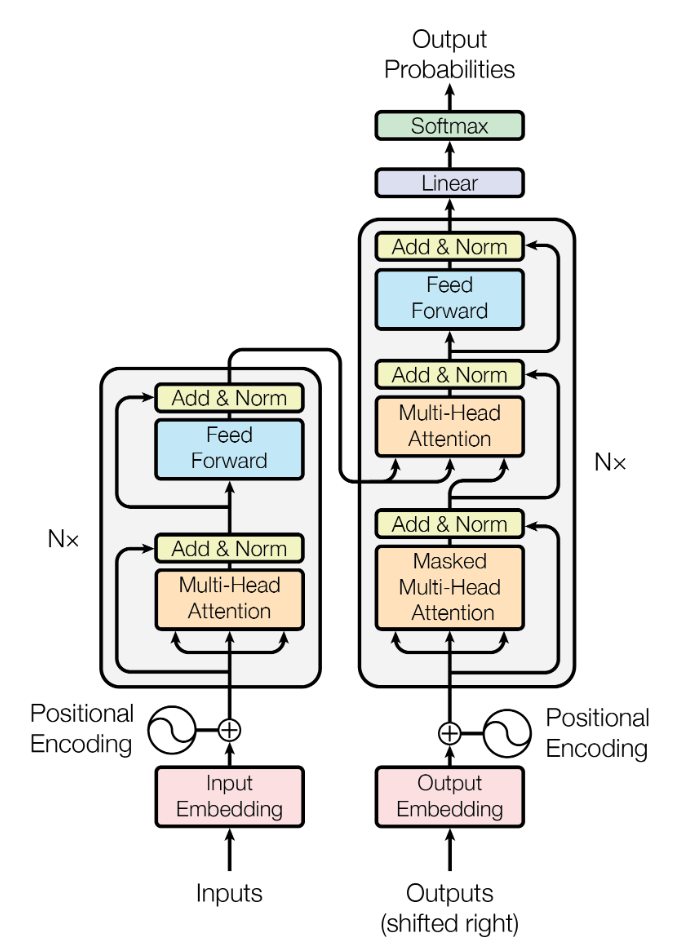
\includegraphics[width=0.5\linewidth]{img/transfomer.png}
  \vspace{0.5cm}
  \caption[Transformer architecture]{Transformer architecture \cite{vaswani2017attention}}
  \label{figure:transformer-architecture}
\end{figure}

As illustrated in Figure \ref{figure:transformer-architecture}, the Transformer follows an encoder-decoder structure \cite{cho2014learning}. The encoder consists of $N$ blocks, each built up by a multi-head attention layer followed by a feedforward layer. The decoder takes the sequence of right-shifted tokens $(\xbf_2,\ldots, \xbf_{N+1})$, masks and processes multi-head attention for themselves, before feeding to other $N$ identical blocks as the encoder, together with the output of the encoder. Final output is a probability distribution for the next token over the dictionary.

The token $\ybf_n, n\in\{1,\ldots,N\}$ is then modified by a linear combination of the values, weighted by the normalized matching scores
$$\ybf_n \leftarrow \ybf_n + \mathrm{softmax}\left(\dfrac{\q_n\mathbf{K}^\top}{\sqrt{d}}\right)V.$$

\subsection{Vision Transformer}
The Transformer architecture is not limited to NLP tasks. Vision Transformer (ViT) is the first work to show that this architecture outperforms traditional Convolutional Neural Networks (CNNs) on image classification tasks \cite{dosovitskiy2020image}. Figure \ref{figure:ViT} illustrated the design of ViT, where each image is divided into patches and treated as a sequence of token which is almost similar to original Transformer.

\begin{figure}
    \centering
    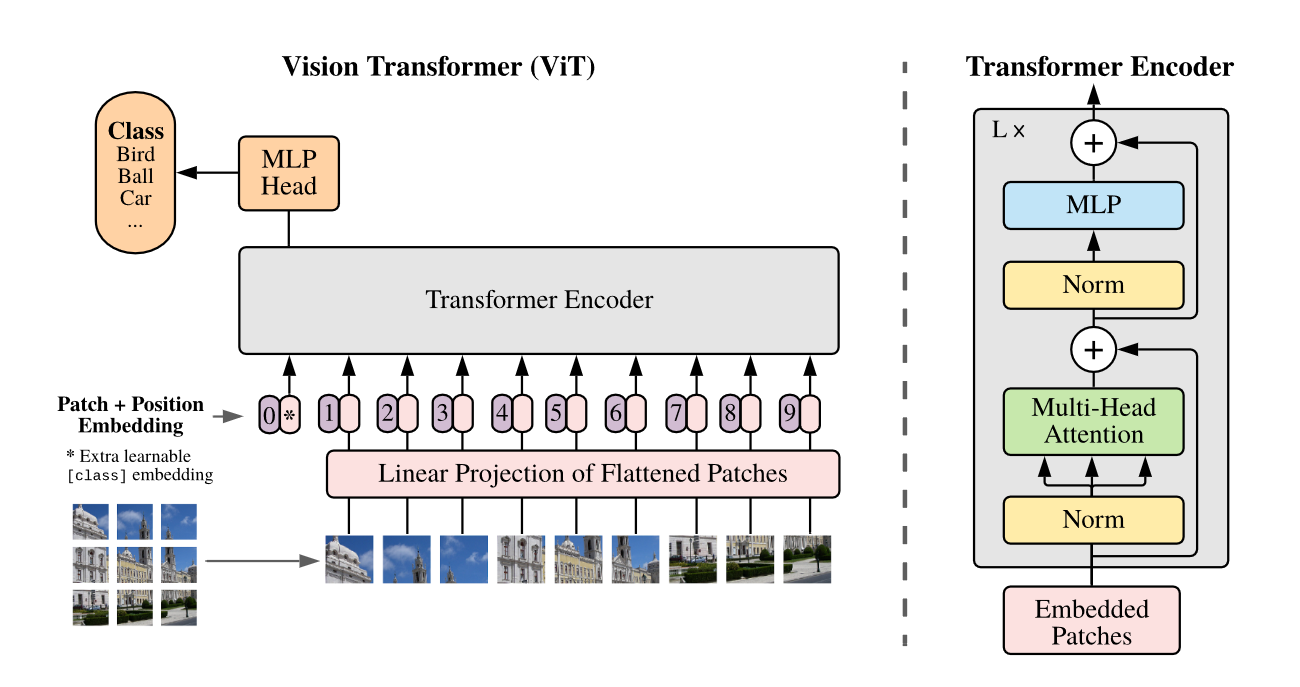
\includegraphics[width=0.8\linewidth]{img/ViT.png}
    \caption[Vision Transformer architecture]{Vision Transformer architecture \cite{dosovitskiy2020image}}
    \label{figure:ViT}
\end{figure}



% \subsection{An Application in Computer Vision}

% \begin{figure}[ht]
%   \centering
%   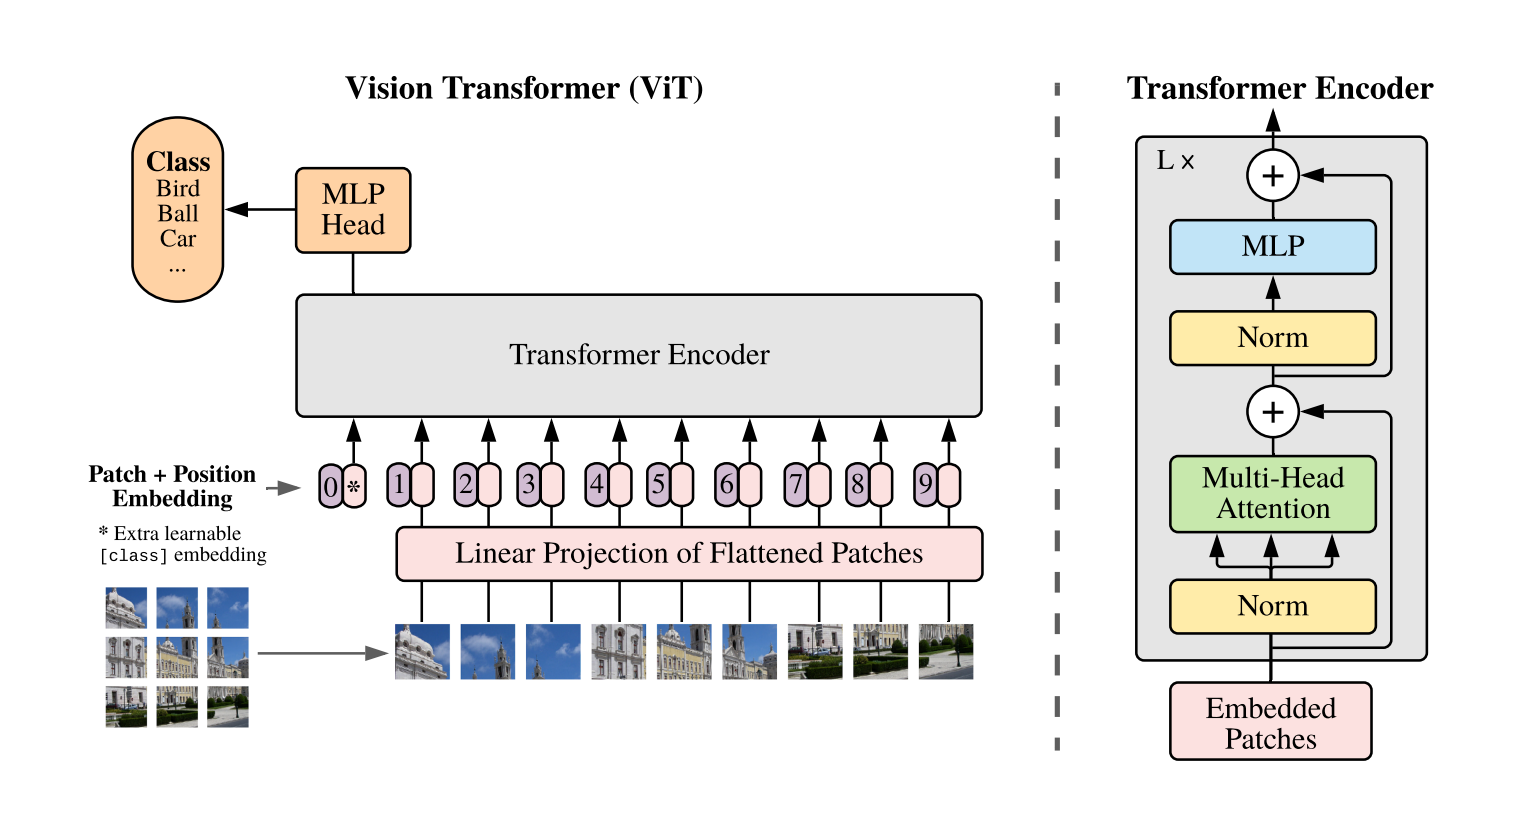
\includegraphics[width=0.75\linewidth]{img/vision-transformer.png}
%   \caption{Vision Transformer Architecture}
%   \label{figure:vision-transformer-architecture}
% \end{figure}

% Note that the number of parameters Attention Mechanism does not depend on the context size $N$. According to the specific problem and dataset, multilayer perceptrons are added for the final output. For generative models, given a sequence of symbols, the expected output is a categorical distribution of symbols in the corpus, to predict the next symbol.

